\documentclass[10pt,journal,cspaper,compsoc]{IEEEtran}

\usepackage{graphicx}
\usepackage[tight,footnotesize]{subfigure}
\usepackage{hyperref}

\title{Swarm: A Lightweight yet Highly Effective Method for Improving Random Testing}

\author{Alex~Groce,~\IEEEmembership{Member,~IEEE,}
        Chaoqiang~Zhang,
        Yang Chen,
        Eric Eide,
        Mohammad Amin Alipour,
        and~John~Regehr~\IEEEmembership{Member,~IEEE,},
\IEEEcompsocitemizethanks{\IEEEcompsocthanksitem A. Groce, C. Zhang, and M. Alipour are with the School of
of Electrical Engineering and Computer Science, Oregon State University, Corvallis, OR, 97331.\protect\\
% note need leading \protect in front of \\ to get a newline within \thanks as
% \\ is fragile and will error, could use \hfil\break instead.
\IEEEcompsocthanksitem Y. Chen, E. Eide, and J. Regehr are with the School of Computing, University of Utah, Salt Lake City, 84112.}% <-this % stops a space
\thanks{}}

\begin{document}

\maketitle

\begin{abstract}
Swarm testing is an approach to improving the effectiveness of random
testing that replaces the traditional testing procedure of generating
tests from a single probability distribution with the use of a
``swarm'' of distributions each of which disallows certain test
behaviors completely.  This paper shows that swarm has two highly
desireable properties.  First, swarm is in many cases extremely
effective, resulting in 40\% or better improvements in \emph{distinct
faults detected} for critical real-world systems such as compilers.
Second, swarm is an encourgagingly \emph{lightweight} method for
improving random testing, with very few demands on would-be users;
applying swarm to an existing random testing system is almost always
trivially easy. In our experience, even a programmer unfamiliar with a
complex testing system can often apply swarm testing to it.  The
widespread applicability and effectiveness of swarm testing suggests a
new domain of random testing research: the search for techniques that
rely only on general features of most test spaces, and do not require
much additional programmer effort or analytical machinery to apply to
already existing random testing frameworks, which are frequently
complex and difficult to modify.  This paper presents case studies
demonstrating the lightweight nature and high effectiveness of swarm
across a set of important real-world case studies.
%
\end{abstract}



%% -*- mode: LaTeX -*-

%%%%%%%%%%%%%%%%%%%%%%%%%%%%%%%%%%%%%%%%%%%%%%%%%%%%%%%%%%%%%%%%%%%%%%%%%%%%%%%

This paper focuses on answering a single question: In random testing,
can a diverse set of \emph{testing configurations} perform better than
a single, possibly ``optimal'' configuration? 
%
An example of a test configuration would be, for example, a list of
API calls that can be included in test cases.
%
Conventional wisdom in random testing~\cite{Hamlet94} has assumed a
policy of finding a ``good'' configuration and running as many tests
as possible with that configuration.
%
Considerable research effort has been devoted to the question of how
to tune a ``good configuration,'' e.g., how to use genetic algorithms
to optimize the \emph{frequency} of various method
calls~\cite{AndrewsL07}, or how to choose a length for
tests~\cite{ASE08}.
%
As a rule, the notion that some test configurations are ``good'' and
that finding a good (if not truly optimal, given the size of the
search space) configuration is important has not been challenged.
Furthermore, in the interests of maximizing coverage and fault
detection, it has been assumed that a good random test configuration
includes as many API calls or other input domain features as possible,
and this has been the guiding principle in large-scale efforts to test
C compilers~\cite{csmith}, file systems~\cite{ICSEDiff}, and utility
libraries~\cite{Pacheco}.  The rare exceptions to this rule have been
cases where a feature makes tests too difficult to evaluate or slow to
execute, or when static analysis or hand inspection can demonstrate
that an API call is unrelated to state~\cite{ICSEDiff}.  For example,
including pointer assertions may make compiling random C programs too
slow with some compilers.

In general, if a call or feature is omitted from some tests, it is
usually omitted from all tests.  This approach seems to make intuitive
sense: omitting features, unless it is necessary, means \emph{giving
up on detecting some faults}.  However, this objection to feature
omission only holds so long as testing is performed using a single
test configuration.  Swarm testing, in contrast, uses a diverse
``swarm'' of test configurations, each of which \emph{deliberately
omits certain API calls or input features}.
%
As a result, given a fixed testing budget, swarm testing tends to test
a more diverse set of inputs than would be tested under a so-called
``optimal'' configuration (perhaps better referred to as a
\emph{default} configuration) in which every feature is available for
use by every test.

One can visualize the impact of swarm testing by imagining a ``test
space'' defined by the contents of tests. As a simple example,
consider testing an implementation of a stack ADT that provides two
operations, push and pop. One can visualize the test space for the
stack ADT using these features as axes: each test is
characterized by the number of times it invokes each operation.
%
Any method for randomly generating test cases results in a probability
distribution over the test space, with the value at each point $(x,y)$ giving
the probability that a given test will contain exactly $x$ pushes and $y$ pops
(in any order).
%
To make this example more interesting, imagine the stack implementation has a
capacity bug, and will crash whenever the stack is required to hold
more than 32~items.


Missing fig illustrates the situation for testing the stack
with a test generator that chooses pushes and pops with equal probability.  The
generator randomly chooses an input length
% (according to a gaussian distribution)
and then decides if each operation is a push or a pop.  The graph shows the
distribution of tests produced by this generator over the test space.  The
graph also shows contour lines for significant regions of the test space.
Where $P_{fail}=1$, a test chosen randomly from that region is certain to
trigger the stack's capacity bug; where $P_{fail}=0$, no test can trigger the
bug.
%
As missing fig shows, this generator only rarely produces
test cases that can trigger the bug.


Now consider a test generator based on swarm testing. This generator
first chooses a non-empty subset of the stack API and then generates a
test case using that subset. 
%
Thus, one-third of the test cases contain both pushes and pops,
one-third just pushes, and one-third just pops.
%
\autoref{fig:stack:swarm} shows the distribution of test cases output by
this generator.  As is evident from the graph, this generator often produces
test cases that trigger the capacity bug.


Although simple, this example illustrates the dynamics that make
swarm testing work.
%
The low dimensionality of the stack example is contrived, of course, and we
certainly believe that programmers should make explicit efforts to test
boundary conditions.
%
As evidenced by the results presented in this paper, however, swarm testing
generalizes to real situations in which there may be dozens of features that
can be independently turned on or off.  It also generalizes to testing real
software in which faults are very well hidden.

Every test generated by any swarm configuration can, in principle, be
generated by a test configuration with all features enabled.
%
However---as the stack example illustrates---the probability of
covering parts of the state space and detecting certain faults can be
demonstrably higher when a diverse set of configurations is tested.


Swarm testing has several important advantages.
%
First, it is low cost: in our experience, existing random test case
generators already support or can be easily adapted to support feature omission.
%
Second, swarm testing reduces the amount of human effort that must be devoted
to tuning the random tester.
%
In our experience, tuning is a significant ongoing burden.
%
Finally---and most importantly---swarm testing makes significantly
better use of a fixed CPU time budget than does random testing using a
single test configuration, in terms of both coverage and fault
detection.
%
For example, we performed an experiment where two machines, differing
only in that one used swarm testing and one did not, used
Csmith~\cite{csmith} to generate tests for a collection
of production-quality C compiler versions for x86-64.
% 
During one week of testing, the swarm machine found 104 distinct ways
to crash compilers in the test suite whereas the other
machine---running the default Csmith test configuration, which enables all
features---found only 73.
%
An improvement of more than 40\% in terms of number of bugs found,
using a random tester that has been intensively tuned for several
years, is surprising and significant.


Even more surprising were some of the details.
%
We found, for example, a compiler bug that could only be triggered by
programs containing pointers, but which was almost never triggered by
inputs that contained arrays.
%
This is odd because pointer dereferences and array accesses are very
nearly the same thing in C\@.\footnote{In C/C++, \texttt{a[i]} is
  syntactic sugar for \texttt{*(a+i)}.}
% 
Moreover, we found another bug in the same compiler that was only
triggered by programs containing arrays, but which was almost never
triggered by inputs containing pointers.
%
Fundamentally, it appears that omitting features while
generating random test cases can lead to improved test effectiveness.


Our contributions are as follows.
%
First, we characterize \emph{swarm testing}, a pragmatic variant of
random testing that increases the diversity of generated test
cases with little implementation effort.
%
The swarm approach to diversity differs from previous methods
in that it focuses solely on \emph{feature omission diversity}:
variance in which possible input features are \emph{not} present in
test cases.
%
Second, we show that---in three case studies---swarm testing offers
improved coverage and bug-finding power.
%
Third, we offer some explanations as to \emph{why} swarm testing works.


\section{SpiderMonkey Results}

\begin{figure*}[t]
  \centering
  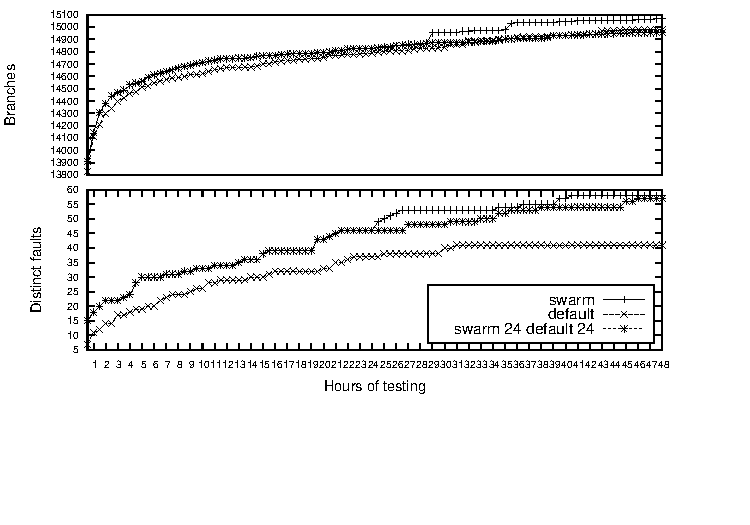
\includegraphics[width=\textwidth]{../graphs/SpiderMonkey/js16}
  \vspace{-1.3in}
  \caption{SpiderMonkey 1.6 Results}
  \label{fig:smonkey16}
\end{figure*}

\begin{figure*}
  \centering
  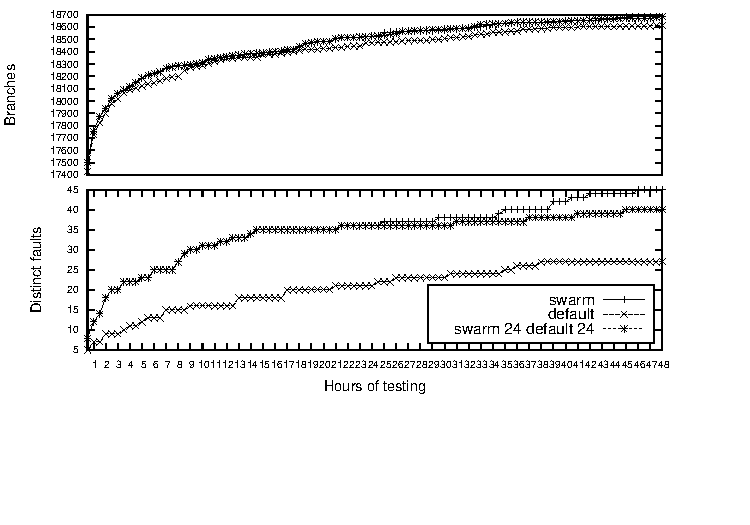
\includegraphics[width=\textwidth]{../graphs/SpiderMonkey/js17}
  \vspace{-1.5in}
  \caption{SpiderMonkey 1.7 Results}
  \label{fig:smonkey17}
\end{figure*}

\begin{figure*}[b]
  \centering
  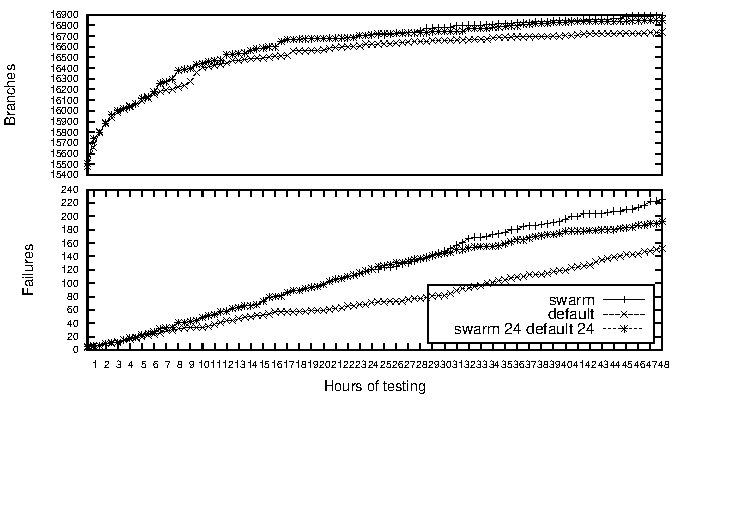
\includegraphics[width=\textwidth]{../graphs/SpiderMonkey/js185}
  \vspace{-1.5in}
  \caption{SpiderMonkey 1.8.5 Results:  Note that this graph shows failures rather than faults.}
  \label{fig:smonkey185}
\end{figure*}

Figures \ref{fig:smonkey16}-\ref{fig:smonkey185} show a comparison
between swarm testing and a default strategy for Mozilla's
SpiderMonkey JavaScript engine, for release versions 1.6, 1.7, and
1.8.5.  Tests were generated using the last public version of the {\tt
jsfunfuzz} JavaScript fuzzing tool~\cite{jsfunfuzz}, both in its
original form and modified to perform swarm testing.  The modification
of {\tt jsfunfuzz} to perform swarm testing was extremely simple.
First, the source code was reformatted with a regular expression to
place individual choices in the random selectors on separate lines.
Second, the reformatted code was ``swarmed'' by a 30 line python
script that removed items in each random choice, with 50\% probability
for each removal.  We estimate that this process took perhaps 30
minutes for a developer unfamilliar with either the {\tt jsfunfuzz}
code or the JavaScript language.

\subsection{Experimental Procedure}

Tests were generated in 30 minute budget runs, and coverage and
faults or failures were computed for each 30 minute run.  The graphs
show cumulative branch coverage and faults or failures for 48 hours of
testing.  In addition to a pure-swarm and pure-default strategy, we
also show results for a strategy that performs swarm testing for 24
hours, then switches to the default configuration, in the hope that
this will explore behaviors hard to reach under swarm.

Distinct faults for versions 1.6 and 1.7 were estimated by using
historical repository data; all faults detected for these versions
were fixed for current versions of SpiderMonkey.  We therefore
performed a search for an identifying $r$ for each test case $t$: $r$
is the revision number of the first commit to the source repository
such that (1) $t$ fails for the version of the code before commit $r$
and (2) $t$ no longer fails once commit $r$ is included.  We assume
commit $r$ fixes $t$ and therefore identifies the underlying fault
exposed by $t$.  This method is obviously approximate. Multiple faults
may be fixed in one commit, or something that we would conceptually
call ``one fault'' may be fixed by multiple partial fixes that do not
completely handle the problem but handle some failing tests (e.g., a
comparison operator such as {\tt > 10} that should be instead {\tt >
8} is changed to {\tt > 9}).  Additionally, a non-fix may sometimes
cause a test to behave differently --- for example, introducing a new
optimization may sometimes cause tests exposing a still-present fault
to no longer trigger it, as the fault-inducing aspect of the compiled
code is removed by the new optimization.  However, hand examination of
a similar method in previous work~\cite{PLDI13} showed that in general
this is a very good approximation of actual faults.  For SpiderMonkey
1.8.5, too few of the discovered faults were clearly fixed in the
latest releases, the source code repository mechanism changed, and the
number of distinct faults appeared to be small enough to make the
uncertainties of this method problematic, so we only measured actual
failures, as these were themselves quite rare for 1.8.5.

\subsection{Results and Statistical Validation}

In order to statistically validate these results, we applied
two-tailed Welch's t-test and Wilcox U-test to the 96 individual
30-minute test blocks for swarm and default.  For all measures (branch
coverage, statement coverage, failures, and faults) and all three
SpiderMonkey versions, the differences between swarm and the default
strategy were statistically significant at the 99\% level (in fact,
the largest $p$-value observed was 0.003 for 1.7 statements).  Table
\ref{tab:effect} shows 95\% confidence interval bounds from the Welch
test on the effect sizes for each measure, for all versions.  Note
that while the absolute difference for failures for 1.8.5 is small,
only 1.6 failures on average were found using the default strategy
during each 30 minute test run, so 0.3 failures is a nearly 19\%
improvement.  The absolute coverage differences represent small
relative improvements, while the small lower bounds on absolute
distinct fault improvements for versions 1.6 and 1.7 are \emph{nearly
40\% and nearly 70\% improvements}, respectively over the default.
While the coverage improvements are also desireable, a 40-70\%
improvement in fault detection for a trivial-to-implement modification
to test generation is the key argument for swarm testing's value.

\begin{table}
\caption{95\% effect sizes (absolute) for swarm over default, SpiderMonkey}

\begin{tabular}{c||c|c|c|c}
\hline
Version & ST & BR & Failures & Faults \\
\hline
\hline
1.6 & 40.4 - 72.0 & 25.8 - 54.0 & 16.3 - 22.4 & 2.6 - 4.9\\
\hline
1.7 & -7.5 - 37.6 & 27.2 - 51.1 & 15.9 - 19.1 & 3.7 - 4.9\\
\hline
1.8.5 & 63.3 - 90.4 & 44.6 - 70.1 & 0.3 - 1.2 & N/A\\
\hline
\end{tabular}
\label{tab:effect}
\end{table}

\subsection{Using Feedback to Improve Swarm}

\begin{figure*}[t]
  \centering
  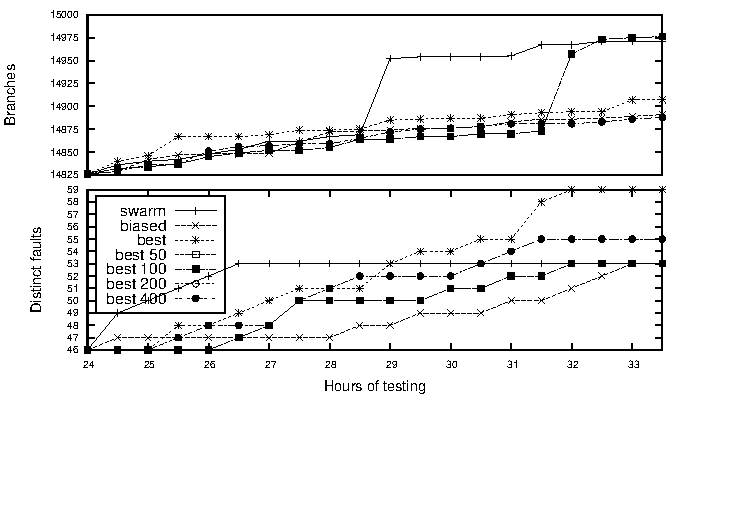
\includegraphics[width=\textwidth]{../graphs/SpiderMonkey/js16strats}
  \vspace{-1.3in}
  \caption{SpiderMonkey 1.6 Feedback Results}
  \label{fig:smonkey16strat}
\end{figure*}

\begin{figure*}
  \centering
  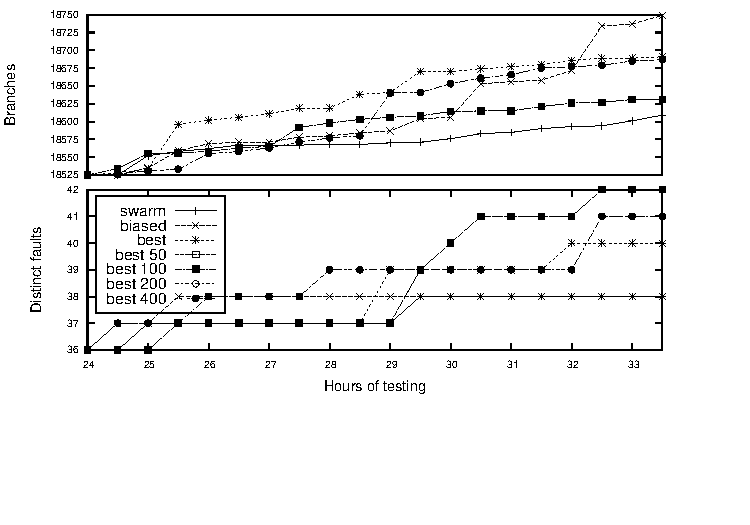
\includegraphics[width=\textwidth]{../graphs/SpiderMonkey/js17strats}
  \vspace{-1.5in}
  \caption{SpiderMonkey 1.7 Feedback Results}
  \label{fig:smonkey17strat}
\end{figure*}

Figures \ref{fig:smonkey16strat} and \ref{fig:smonkey17strat} show the
results of attempting to exploit the results of the first 24 hours of
swarm testing to improve testing for the next 24 hour period, tuning
the configurations used.  

Because measuring code coverage after each test is expensive, we used
a feedback approach based on coverage over difficult-to-execute
coverage entities only.  We considered a branch or line
``uninteresting'' if it was executed during every 30 minute run in the
first 24 hours of testing.  Coverage for the remaining ``interesting''
blocks and branches only was collected for each test, and
ranked configurations by the total value (the log of the inverse of
the frequency of coverage over all tests) of all covered entities.
The feedback strategies were then (1) to re-use the best (or best 50,
100, 200, or 400) configurations in round-robin fashion for future
test generation, and (2) to include each feature with a biased
non-50\% probability based on its frequency in tests executing at least
one interesting coverage entity.

While some strategies show a cumulative improvement on swarm in terms
of coverage or fault detection, \emph{no improvements} (measured in
terms of 30 minute run improvements on the cumulative swarm coverage
at 24 hours) are statistically significant; in some cases there was a
statistically significant \emph{reduction} in new distinct faults per
run.  The results were similar enough to the pure swarm strategy, and
required sufficient computational effort (in computing detailed
coverage results and ranking configurations) and additional test
infrastructure development that we find little support for applying
simple feedback mechanisms.  It is possible more sophisticated
methods, e.g. using machine learning, may be valuable, but the most
important goal would be to cover \emph{never-executed} code, for which
there is, in general, no data from which learn a good configuration.
Our hypothesis was that executing infrequently executed code more
often should lead to either detection of bugs concerning that code, or
execution of ``nearby'' uncovered code.  While feedback did indeed
increase the frequency of rarely executed entities, it did not produce
a clear effect in terms of bugs or novel coverage.


\section{YAFFS2 Results}

\begin{figure*}[t]
  \centering
  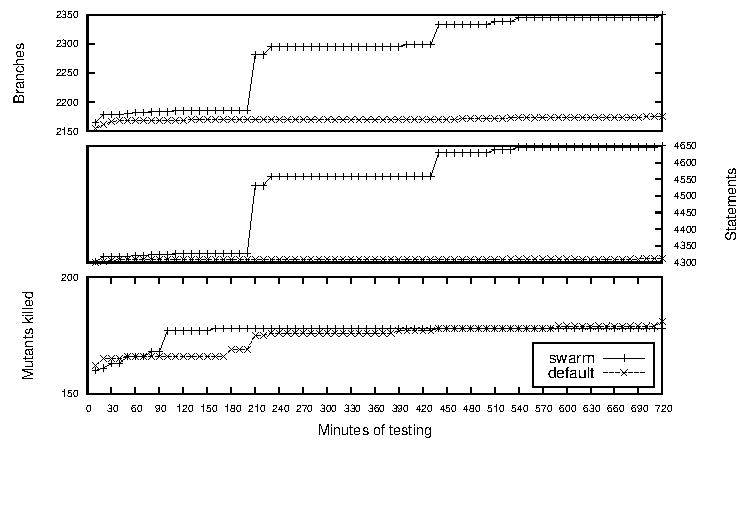
\includegraphics[width=\textwidth]{../graphs/yaffs2/yaffs2}
  \vspace{-1.3in}
  \caption{YAFFS2 Results}
  \label{fig:yaffs2}
\end{figure*}

YAFFS2~\cite{yaffs2} is a popular open-source NAND flash file system
for embedded use; it was the default image format for early versions
of the Android operating system.  The test generator for YAFFS uses 47
different API calls as features.  Applying swarm testing to YAFFS2 was
essentially trivial, as the capability to turn on or off API calls is
natural to such API-based random test generators; we did refactor the
control from a {\tt \#define} based approach to command-line
parameters to ease use of swarm testing.

Figure \ref{fig:yaffs2} shows that swarm testing improves not only
branch and statement coverage but also mutation kill rates for YAFFS2.
Because YAFFS2 is a smaller and simpler program than SpiderMonkey, we
used 10 minute rather than 30 minute test intervals.  All differences
between swarm and default testing were statistically significant by
Wilcox U-test for the 10 minute intervals, with $p$-values of $3.1
\times 10^7$ or lower.  Tables \ref{tab:yaffseffect} summarizes 95\%
confidence interval absolute gains in coverage and mutation kill for 10 minutes of swarm testing vs. 10 minutes of default testing.

\begin{table}
\caption{95\% effect sizes (absolute) for swarm over default, YAFFS2}
\centering
\begin{tabular}{c|c|c}
\hline
ST & BR & Mutants Killed \\
\hline
\hline
15.7 - 50.1 & 10.5 - 28.1 \\
\hline
\end{tabular}

\label{tab:yaffseffect}
\end{table}


%% -*- mode: LaTeX -*-
%%

%%%%%%%%%%%%%%%%%%%%%%%%%%%%%%%%%%%%%%%%%%%%%%%%%%%%%%%%%%%%%%%%%%%%%%%%%%%%%%%

\section{Conclusion}

Swarm testing relies on the following claim: for realistic systems,
\emph{randomly excluding some features from some tests} can improve
coverage and fault detection, compared to a test suite that
potentially uses every feature in every test.
%
The benefit of using of a single, inclusive, default
configuration---that every test can potentially expose any fault and
cover any behavior, heretofore usually taken for granted in random
testing---does not, in practice, make up for the fact that \emph{some
features can, statistically, suppress behaviors.}  Effective testing
therefore may require feature omission diversity.
%
We show that this not only holds for simple container-class examples
(e.g., pop operations suppress stack overflow) but for a widely used
flash file system and 14 out of 17 versions of five production-quality C
compilers.
%
For these real-world systems, if we compare testing with a single
inclusive configuration to testing with a set of 100--1,000
unique configurations, each omitting features with 50\% probability
per feature, we have observed (1)~significantly better fault
detection, (2)~significantly better branch and statement coverage, and
(3)~strictly superior mutant detection.  
%
Test configuration diversity does indeed produce better testing in
many realistic situations.


Swarm testing was inspired by swarm verification, and we hope that its
ideas can be ported back to model checking.
%
We also plan to investigate swarm in the context of bounded exhaustive
testing and learning-based testing methods.
%
Finally, we believe there is room to better understand \emph{why}
swarm provides its benefits, particularly in the context
of large, idiosyncratic SUTs such as compilers, virtual machines, and
OS kernels.
%
More case studies will be needed to generate data to support this
work.  We also plan to investigate how swarm testing's increased
diversity of code coverage in test cases can benefit fault
localization and program understanding algorithms
relying on test cases~\cite{Tarantula}; traditional random tests are far more
homogeneous than swarm tests.


We have made Python scripts supporting swarm testing available at
\url{http://beaversource.oregonstate.edu/projects/cswarm/browser/release}.
%
%% ENE: cut for space.
%
% The {\tt genconfigs} tool supports Gaussian distributions of numeric
% parameters and feature dependencies as well as the binary
% inclusion/omissions used in this paper.

%%%%%%%%%%%%%%%%%%%%%%%%%%%%%%%%%%%%%%%%%%%%%%%%%%%%%%%%%%%%%%%%%%%%%%%%%%%%%%%

%% End of file.


\bibliographystyle{IEEEtran}

\bibliography{bibliography}

\end{document}